\chapter{Conception du Systeme}

\section{Architecture Globale}

Le systeme Moroccan Legal RAG est concu selon une architecture modulaire en couches, ou chaque composant est independant et communicant via des interfaces bien definies. L'architecture suit le paradigme RAG (Retrieval-Augmented Generation) avec une strategie de recherche hybride associant similarite semantique dense et recherche lexicale BM25.

\subsection{Vue d'Ensemble}

L'architecture globale s'articule autour de cinq couches principales :

\begin{enumerate}
    \item \textbf{Couche Ingestion} : Extraction du texte depuis les documents sources (PDF), correction OCR, nettoyage, normalisation arabe, et structuration en articles.
    \item \textbf{Couche Stockage} : Base de donnees PostgreSQL 16 avec l'extension pgvector 0.7.4 pour le stockage des articles et de leurs vecteurs semantiques (embeddings).
    \item \textbf{Couche Recherche} : Moteur de recherche hybride combinant similarite cosinus (dense) et BM25 avec tokenizer arabe specialise, fusionnes par Reciprocal Rank Fusion (RRF).
    \item \textbf{Couche Generation} : Modele de langage Gemma 4 (2B parametres, quantifie Q4\_K\_XL GGUF) pour la generation de reponses juridiques ancrees dans les articles retrouves.
    \item \textbf{Couche Presentation} : API REST (FastAPI), interface web (SvelteKit 5 + Tailwind CSS 4), et interface terminal (Textual).
\end{enumerate}

\begin{figure}[H]
    \centering
    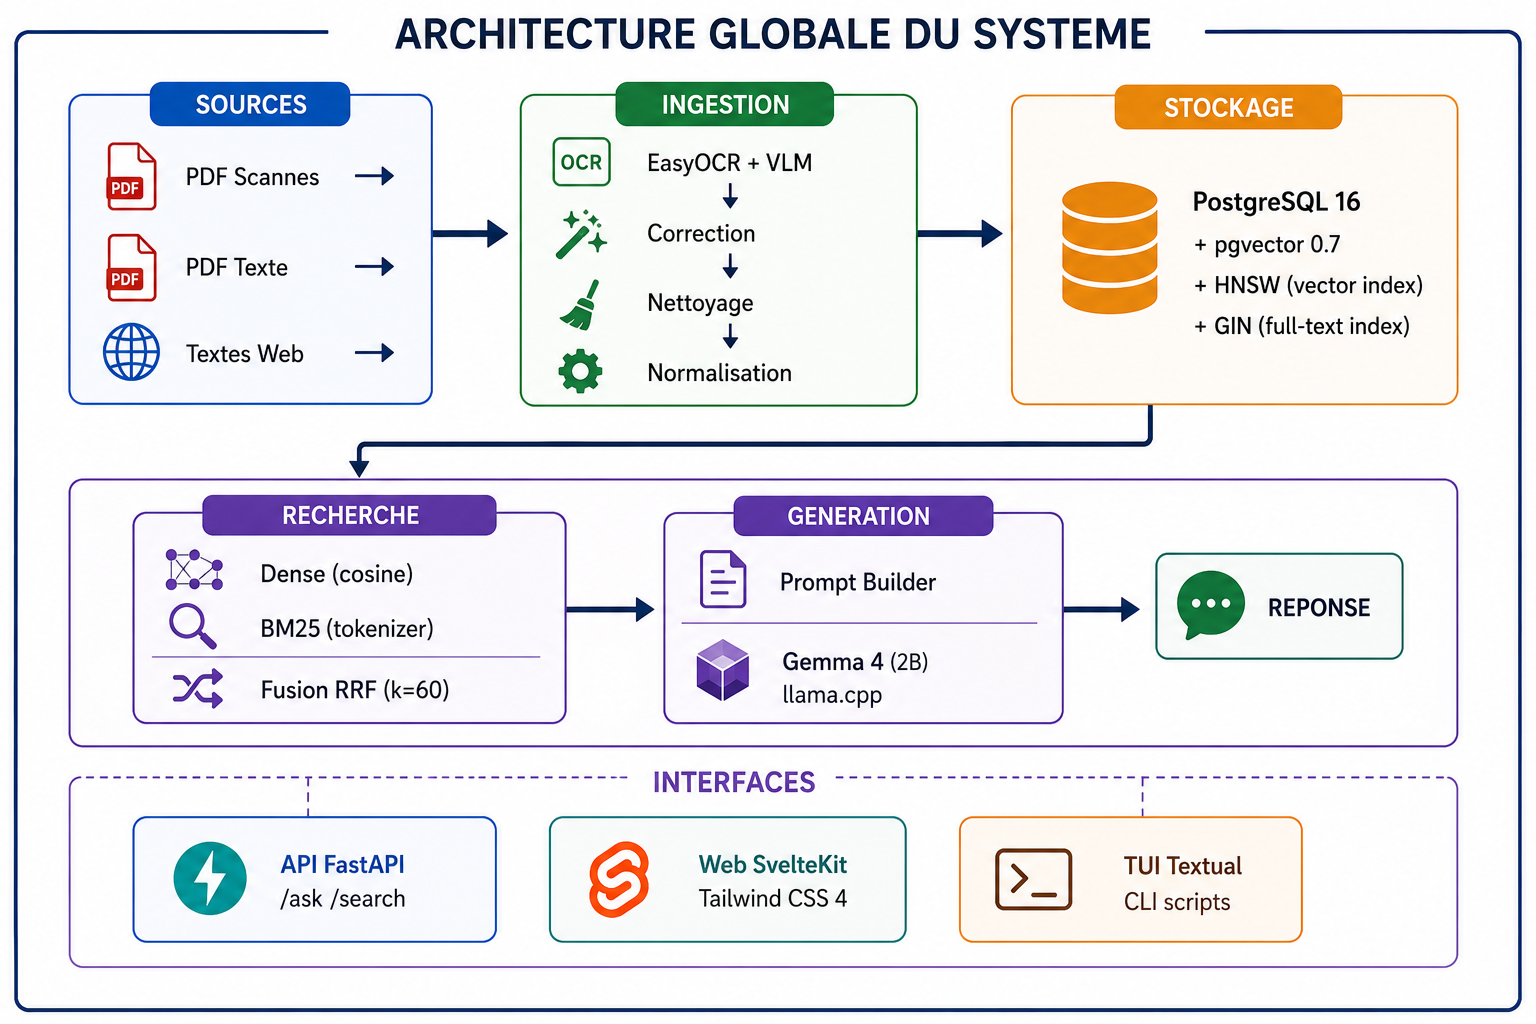
\includegraphics[width=\textwidth]{images/illustrations/architecture_globale_systeme.png}
    \caption{Overall architecture of the legal RAG system, showing the document ingestion workflow, storage layer, hybrid retrieval engine, response generation pipeline, and user-facing interfaces.}
    \label{fig:global-architecture}
\end{figure}

La Figure~\ref{fig:flux-donnees} (Section~\ref{sec:flux-donnees}) detaille le cheminement complet d'une requete a travers ces couches.

\subsection{Stack Technique Detaillee}

Le tableau~\ref{tab:stack-technique} resume les technologies retenues pour chaque couche du systeme :

\begin{table}[h]
\centering
\renewcommand{\arraystretch}{1.3}
\begin{tabular}{|l|l|l|}
\hline
\rowcolor{LightBlue}
\textbf{\color{PrimaryBlue}Couche} & \textbf{\color{PrimaryBlue}Technologie} & \textbf{\color{PrimaryBlue}Role} \\
\hline
Extraction PDF & PyMuPDF, pdfplumber & Rendu et extraction de texte \\
OCR & EasyOCR (GPU) & Reconnaissance de l'arabe imprime \\
Correction OCR & Gemma 4 (mode VLM) & Correction des erreurs de reconnaissance \\
Nettoyage & LegalTextCleaner & Suppression bruit structurel \\
Normalisation & ArabicNormalizer & Unification alef, tatweel, diacritiques \\
Structuration & LegalStructureParser & Decoupage en articles avec metadonnees \\
\hline
Embedding & E5-large (1024d, 560M) & Vectorisation semantique des articles \\
Base de donnees & PostgreSQL 16 + pgvector 0.7.4 & Stockage articles + vecteurs \\
Index vectoriel & HNSW (m=16) & Recherche par similarite rapide \\
Index lexical & BM25Okapi + tokenizer arabe & Recherche par mots-cles \\
\hline
Fusion & RRF (k=60) & Combinaison dense + lexical \\
Generation & Gemma 4 2B (Q4\_K\_XL GGUF) & Reponses juridiques en arabe \\
Inference LLM & llama.cpp & CPU + GPU hybride \\
Service distant & Cloudflare Tunnel & Exposition Colab GPU \\
\hline
API & FastAPI (Python) & Endpoints REST \\
Frontend Web & SvelteKit 5 + Tailwind CSS 4 & Interface utilisateur \\
TUI & Textual (Python) & Gestion du corpus en terminal \\
Infrastructure & Docker Compose & Conteneurisation \\
\hline
\end{tabular}
\caption{Stack technique complete du systeme Moroccan Legal RAG}
\label{tab:stack-technique}
\end{table}

\section{Flux de Donnees Principal}
\label{sec:flux-donnees}

Le flux de donnees decrit le cheminement d'une question utilisateur depuis sa soumission jusqu'a la generation de la reponse juridique (Figure~\ref{fig:flux-donnees}) :

\begin{figure}[h]
    \centering
    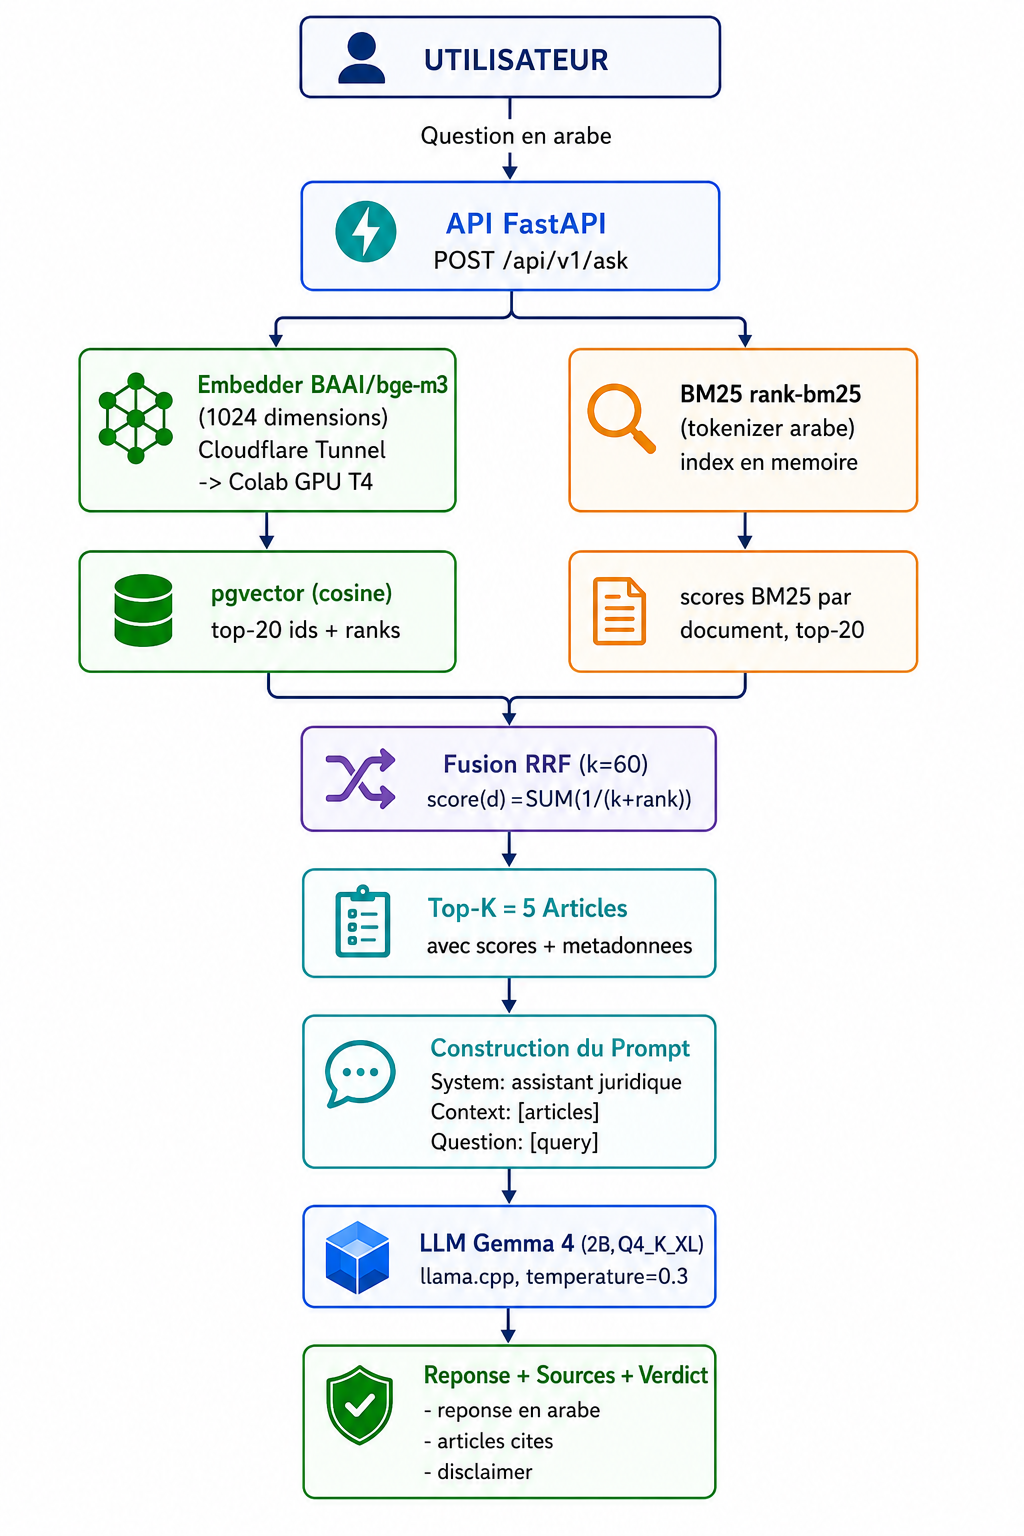
\includegraphics[width=0.85\textwidth]{images/illustrations/rag_dataflow_bge_m3.png}
    \caption{End-to-end data flow of the legal RAG system, combining dense retrieval using BAAI/bge-m3 embeddings and sparse BM25 retrieval through Reciprocal Rank Fusion (RRF) before answer generation with Gemma 4.}
    \label{fig:flux-donnees}
\end{figure}

\section{Phase 1 -- Collecte et Constitution du Corpus}

\subsection{Sources de Donnees}

Le corpus juridique marocain a ete constitue a partir de trois types de sources :

\begin{itemize}
    \item \textbf{Bulletins Officiels (PDF numerises)} : Publication officielle des textes de loi au Maroc. Ces documents sont des scans de qualite variable necessitant une etape d'OCR.
    \item \textbf{PDF natifs} : Certains textes recents sont disponibles en format PDF avec texte selectionnable, permettant une extraction directe.
    \item \textbf{Portails gouvernementaux} : Textes publies sur les sites du SGG, du Ministere de la Justice, et d'ADALA.
\end{itemize}

\subsection{Pipeline d'Extraction}

Le pipeline d'extraction (Figure~\ref{fig:pipeline-extraction}) automatise le passage du PDF brut a l'article structure :

\begin{figure}[H]
    \centering
    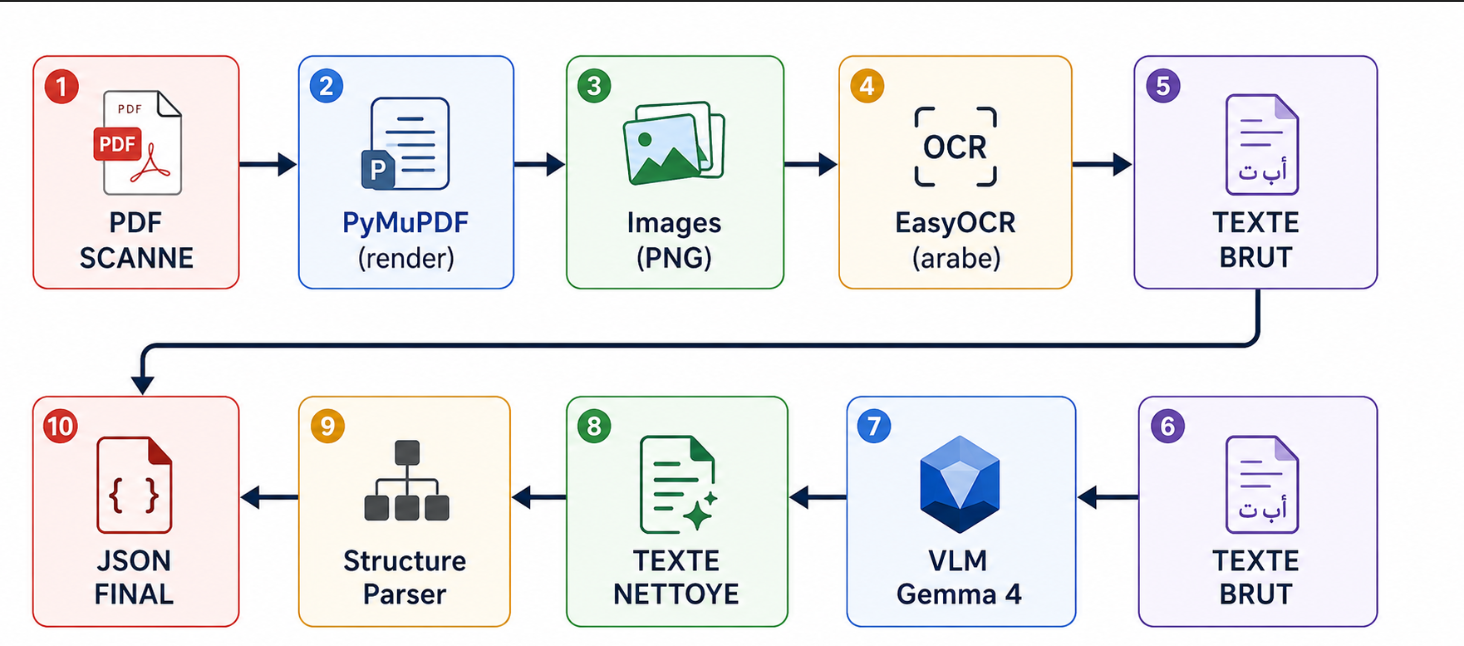
\includegraphics[width=\textwidth]{images/illustrations/pipeline_extraction.png}
    \caption{Document extraction pipeline transforming scanned PDF files into structured JSON articles through OCR, text cleaning, vision-language processing, and schema parsing.}
    \label{fig:pipeline-extraction}
\end{figure}

\subsection{Etapes du Pipeline}

\begin{enumerate}
    \item \textbf{Rendu PDF} : PyMuPDF (fitz) convertit chaque page du PDF en image PNG.
    \item \textbf{OCR} : EasyOCR effectue la reconnaissance du texte arabe sur les images.
    \item \textbf{Correction VLM} : Gemma 4 en mode vision corrige les erreurs de reconnaissance avec un prompt specialise (\textit{«~Corrige UNIQUEMENT les erreurs d'OCR. NE TRADUIS PAS. NE RESUMES PAS.~»}).
    \item \textbf{Nettoyage structurel} : LegalTextCleaner supprime les en-tetes, pieds de page, numeros de page, et les artefacts de numerisation.
    \item \textbf{Normalisation arabe} : ArabicNormalizer unifie les variantes de caracteres (alefs, tatweel, diacritiques) et applique la normalisation Unicode NFKC.
    \item \textbf{Structuration} : LegalStructureParser detecte les motifs \textit{«~\textarabic{المادة} $X$~»} pour delimiter les articles et extraire les metadonnees (chapitre, section, loi).
    \item \textbf{Export JSON} : Chaque article est exporte au format JSON structure avec metadonnees.
\end{enumerate}

\subsection{Structure d'un Article (JSON)}

Chaque article du corpus est represente par le schema JSON du Listing~\ref{lst:article-json} :

\begin{jsonblock}{Document JSON --- Exemple d'article indexé}
\{\\
\quad "article\_number": "513",\\
\quad "law\_name": "code penal maroc ar",\\
\quad "domain": "criminal",\\
\quad "chapter\_title": "\textarabic{حماية الاحداث}",\\
\quad "section\_title": "\textarabic{التدابير الوقائية}",\\
\quad "text": "\textarabic{يعتبر الحدث البالغ من العمر اقل من 16 سنة...}",\\
\quad "source\_file": "code-penal-maroc-ar.pdf",\\
\quad "page\_number": 145\\
\}
\end{jsonblock}
\label{lst:article-json}
\subsection{Corpus Constitue}

Le corpus final est organise par domaine juridique et totalise environ 2\,357 articles (Tableau~\ref{tab:corpus-domaines}) :

\begin{table}[h]
\centering
\renewcommand{\arraystretch}{1.3}
\begin{tabular}{|l|r|r|}
\hline
\rowcolor{LightBlue}
\textbf{\color{PrimaryBlue}Domaine} & \textbf{\color{PrimaryBlue}Articles} & \textbf{\color{PrimaryBlue}Lois principales} \\
\hline
Droit Penal & 822 & Code Penal, Code des Sanctions \\
Circulation & 228 & Code de la Route \\
Droit Civil & 705 & Code des Obligations, Procedure Civile, Impots \\
Droit Commercial & 359 & Registre du Commerce, Droit des Societes \\
Organisation Judiciaire & 32 & Loi 38.15, Carte Judiciaire \\
Droit Fiscal & 211 & Code General des Impots 2024 \\
\hline
\textbf{Total} & \textbf{2\,357} & \\
\hline
\end{tabular}
\caption{Repartition du corpus par domaine juridique}
\label{tab:corpus-domaines}
\end{table}

\section{Phase 2 -- Traitement et Validation des Donnees}

\subsection{Module de Nettoyage (LegalTextCleaner)}

Le module de nettoyage elimine le bruit structurel du texte extrait avant la normalisation linguistique. Il applique les regles suivantes, configurables via \texttt{config/cleaning.yaml} :

\begin{itemize}
    \item Suppression des en-tetes et pieds de page recurrents
    \item Normalisation des espaces et suppression des lignes vides
    \item Correction des retours a la ligne intempestifs en milieu de phrase
    \item Suppression des caracteres parasites de numerisation
    \item Detection et suppression des filigranes (\textit{watermarks})
    \item Deduplication des paragraphes repetes
\end{itemize}

\subsection{Module de Normalisation Arabe (ArabicNormalizer)}

Le normaliseur arabe standardise le texte au niveau des caracteres pour reduire la variabilite et ameliorer la qualite de l'embedding et de la recherche lexicale. Les regles appliquees incluent :

\begin{itemize}
    \item \textbf{Normalisation Unicode NFKC} : Uniformisation des codages equivalents
    \item \textbf{Unification des alefs} : \textarabic{أ}, \textarabic{إ}, \textarabic{آ} $\to$ \textarabic{ا}
    \item \textbf{Suppression du tatweel} : \textarabic{ـ} (kashida) supprime
    \item \textbf{Suppression des diacritiques} : Sauf \textit{shadda} (\textarabic{ّ}) preservee en option
    \item \textbf{Unification de la ponctuation} : Standardisation des separateurs
    \item \textbf{Unification des chiffres} : Chiffres arabo-indiens $\to$ chiffres ASCII
\end{itemize}

\subsection{Module de Structuration (LegalStructureParser)}

Le parser de structure identifie la hierarchie du document juridique :

\begin{itemize}
    \item \textbf{Niveau Article} : Motif \textit{«~\textarabic{المادة} $X$~»} -- delimite chaque article
    \item \textbf{Niveau Chapitre} : Motif \textit{«~\textarabic{الباب} $Y$~»} -- regroupe les articles
    \item \textbf{Niveau Section} : Motif \textit{«~\textarabic{القسم} $Z$~»} -- subdivision du chapitre
    \item \textbf{Niveau Livre} : Motif \textit{«~\textarabic{الكتاب} $W$~»} -- division majeure du code
\end{itemize}

Chaque article herite des metadonnees de son contexte hierarchique (chapitre, section, livre), facilitant la recherche contextuelle.

\subsection{Defis et Solutions}

Les defis rencontres lors du traitement des documents juridiques marocains et les solutions appliquees sont synthetises dans le Tableau~\ref{tab:defis-solutions} :

\begin{table}[h]
\centering
\renewcommand{\arraystretch}{1.3}
\begin{tabular}{|p{3.5cm}|p{3.5cm}|p{4.5cm}|}
\hline
\rowcolor{LightBlue}
\textbf{\color{PrimaryBlue}Probleme} & \textbf{\color{PrimaryBlue}Cause} & \textbf{\color{PrimaryBlue}Solution} \\
\hline
Bruit OCR & Scans de qualite degradee & Correction VLM + regles de nettoyage \\
Texte duplique & Repetitions dans les PDF sources & Detection par hash MD5 + similarite cosinus \\
Melange arabe/francais & Documents multilingues & Segmentation par detection de script Unicode \\
Metadonnees manquantes & Absence de structure explicite & Inference par heuristiques (motifs dans le texte) \\
Formatage irregulier & Heterogeneite des sources & Normalisation configurable via YAML \\
\hline
\end{tabular}
\caption{Defis rencontres et solutions appliquees lors du traitement des donnees}
\label{tab:defis-solutions}
\end{table}

\section{Modelisation de la Base de Donnees}

\subsection{Choix de PostgreSQL + pgvector}

Le choix de PostgreSQL 16 avec l'extension pgvector 0.7.4 repose sur plusieurs criteres decisifs :

\begin{itemize}
    \item \textbf{Unification} : Un seul systeme pour les donnees relationnelles (articles, metadonnees, conversations) et vectorielles (embeddings).
    \item \textbf{Transactions ACID} : Garantie de coherence entre l'insertion d'un article et son embedding.
    \item \textbf{Indexation HNSW} : Recherche vectorielle haute performance (m=16, ef\_construction=200).
    \item \textbf{Full-text search} : Bien que limite pour l'arabe, le tsvector PostgreSQL reste utile pour les metadonnees en francais.
    \item \textbf{Maturite et outillage} : 30+ ans d'existence, pgAdmin, pg\_dump, replication.
\end{itemize}

\subsection{Schema de la Base de Donnees}

Le schema de la base de donnees \texttt{legal\_rag} est presente dans la Figure~\ref{fig:schema-db} :

\begin{figure}[H]
\centering
\centering
    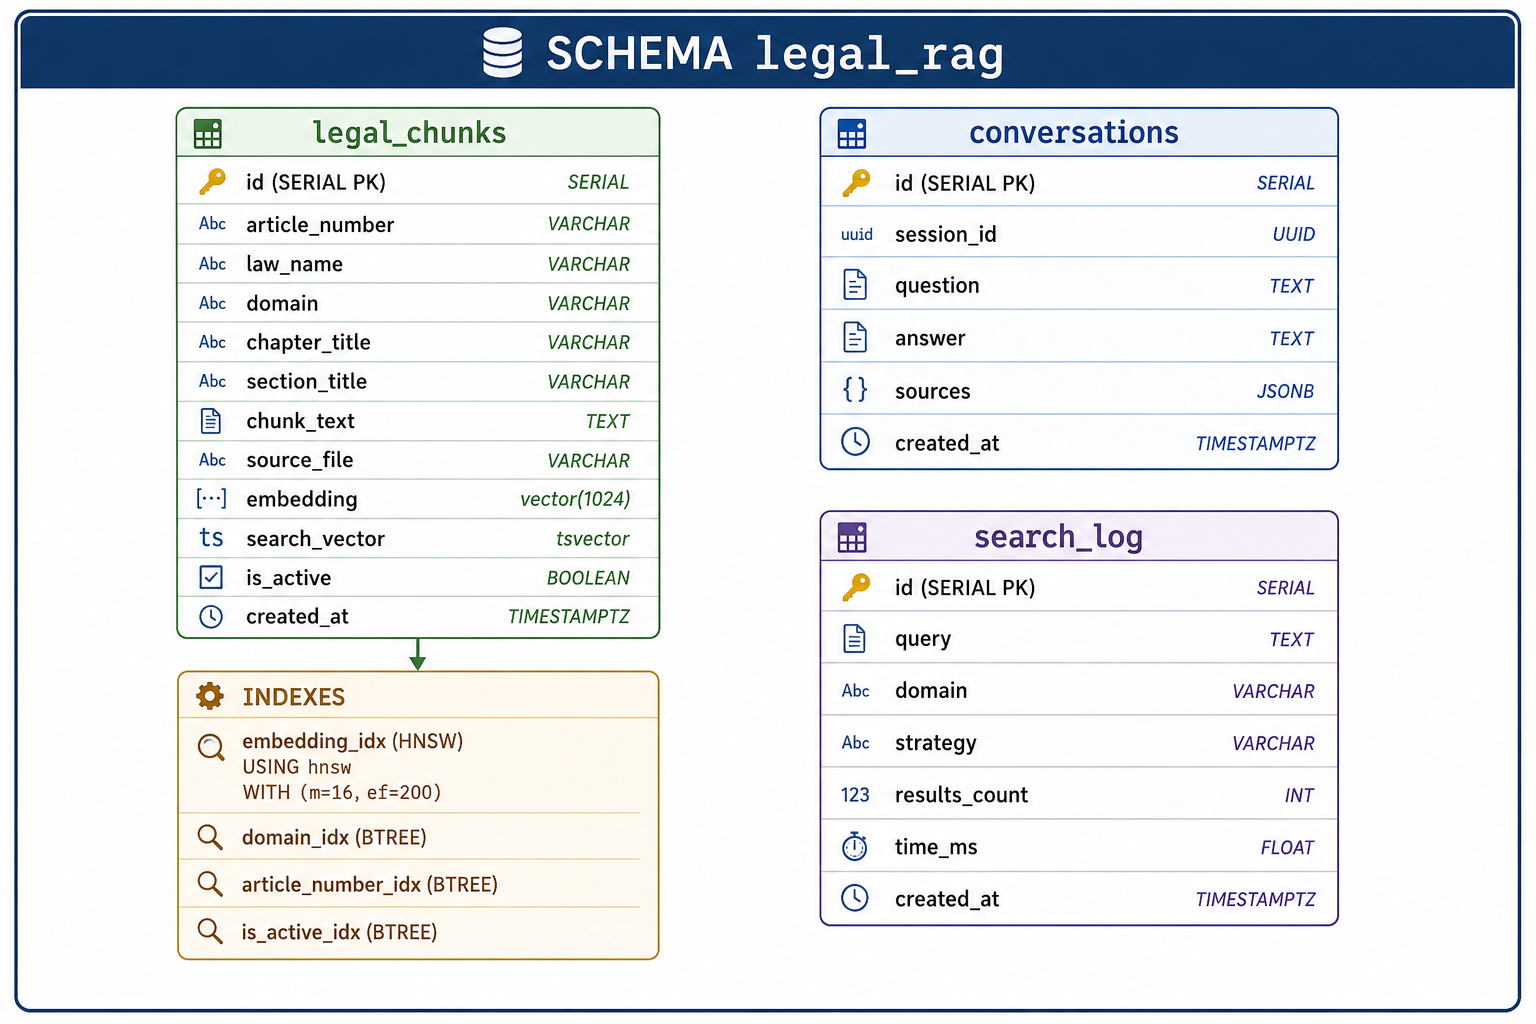
\includegraphics[width=0.95\textwidth]{images/illustrations/legal_rag_schema.png}
    \caption{Schema de la base de donnees \texttt{legal\_rag} avec la table principale \texttt{legal\_chunks} et ses index}
\label{fig:schema-db}
\end{figure}

\subsection{Configuration de l'Index HNSW}

L'index HNSW (Hierarchical Navigable Small World) est configure pour optimiser le compromis entre vitesse de recherche et precision :

\begin{itemize}
    \item \textbf{m = 16} : Nombre de connexions par noeud (valeurs typiques : 16-64). Une valeur de 16 offre un bon compromis pour $\sim$2\,400 vecteurs.
    \item \textbf{ef\_construction = 200} : Taille de la liste dynamique lors de la construction de l'index. Plus la valeur est elevee, plus l'index est precis mais plus sa construction est lente.
    \item \textbf{ef\_search = 100} : Taille de la liste lors de la recherche. Reglable par session.
    \item \textbf{Operateur cosine} : Similarite cosinus, adaptee aux embeddings normalises E5-large.
\end{itemize}

\subsection{Recherche Lexicale BM25}

Suite a l'echec du full-text search PostgreSQL pour l'arabe (0 resultat sur 32 requetes de test, cf. Section~\ref{sec:resultats}), une implementation alternative a ete developpee :

\begin{itemize}
    \item \textbf{Bibliotheque} : rank-bm25 (BM25Okapi) en Python
    \item \textbf{Tokenisation} : Tokenizer arabe specialise avec expression reguliere Unicode, 60+ stop words juridiques, et filtrage des tokens courts ($\ge 2$ caracteres)
    \item \textbf{Normalisation} : Application prealable de l'ArabicNormalizer sur les documents et les requetes
    \item \textbf{Chargement} : Index integral en memoire au premier appel (lazy loading)
\end{itemize}

\section{Deploiement Docker}

L'infrastructure est conteneurisee via Docker Compose avec deux services principaux (Listing~\ref{lst:docker-compose}) :

\begin{verbatim}
# docker-compose.yaml (extrait)
services:
  postgres:
    build:
      dockerfile: docker/Dockerfile.postgres
      args:
        PG_MAJOR: 16
        PGVECTOR_VERSION: 0.7.4
    container_name: legal-rag-postgres
    environment:
      POSTGRES_DB: legal_rag
      POSTGRES_USER: legal_rag_user
    ports:
      - "5432:5432"
    volumes:
      - postgres_data:/var/lib/postgresql/data
      - ./database/init_db.sql:/docker-entrypoint-initdb.d/01-init.sql
    healthcheck:
      test: ["CMD-SHELL", "pg_isready -U legal_rag_user -d legal_rag"]
    deploy:
      resources:
        limits:
          memory: 2G
          cpus: '2'

  pgadmin:
    image: dpage/pgadmin4:latest
    ports:
      - "5050:80"
\end{verbatim}
\label{lst:docker-compose}

L'image PostgreSQL est construite sur mesure pour inclure l'extension pgvector 0.7.4. Le script \texttt{init\_db.sql} est execute automatiquement au premier demarrage pour creer les tables, les index, et les contraintes.

\section{Conclusion de la Conception}

La conception du systeme Moroccan Legal RAG repose sur trois principes directeurs :

\begin{enumerate}
    \item \textbf{Modularite} : Chaque composant (extraction, nettoyage, embedding, recherche, generation) est independant et interchangeable, facilitant l'evolution et la maintenance.

    \item \textbf{Optimisation pour l'arabe juridique} : Chaque etape du pipeline est adaptee aux specificites de l'arabe (normalisation, tokenisation, embedding multilingue) et du domaine juridique (structure en articles, metadonnees hierarchiques, citations).

    \item \textbf{Deploiement leger} : L'utilisation de la quantification GGUF pour le LLM, de l'indexation HNSW pour les vecteurs, et de la conteneurisation Docker permet un deploiement sur du materiel modeste sans compromettre les performances.
\end{enumerate}